\documentclass[conference]{IEEEtran}
\usepackage[pdftex]{graphicx}
\usepackage{url}

% correct bad hyphenation here
\hyphenation{op-tical net-works semi-conduc-tor}

\begin{document}
\title{Asynchronous Arbitration Primitives\\for New Generation of Circuits and Systems}

\author{\IEEEauthorblockN{Andrey Mokhov\IEEEauthorrefmark{1}, Victor Khomenko, Danil Sokolov, Alex Yakovlev}
\IEEEauthorblockA{Newcastle University, Newcastle upon Tyne, United Kingdom}
\IEEEauthorblockA{\IEEEauthorrefmark{1}\emph{Corresponding author:} \url{andrey.mokhov@ncl.ac.uk}}}

\maketitle

\begin{abstract}
This paper presents an overview of a family of asynchronous arbitration
primitives designed to increase the resilience and efficiency of
the new generation of circuits and systems. We cover primitives for
interfacing analog and digital worlds, sampling of non-persistent
signals, and efficient handling of correlated sensor events.
\end{abstract}

% no keywords

\section{Introduction}

Multiple timing and voltage domains\\
Clocked vs async\\
Analog vs digital\\
A2A component\\
Formal methods\\
EDA support\\

\subsection{STG specification language}

Brief description\\

Input/internal/output convention\\

Signal transition loop\\

Handshake\\

Dummy\\

\section{Synchronisation primitives}

In this section we cover \emph{synchronisation primitives} that are used to
isolate asynchronous control logic from potentially hazardous environment.

\subsection{\textsf{WAIT} and \textsf{WAIT0}}

The \textsf{WAIT} element, shown in Fig.~\ref{fig:wait}(left), synchronises the
asynchronous handshake \textsf{ctrl/san}\footnote{The name \textsf{san} stands
for `sanitised', emphasising the role of the element: the output \textsf{san}
is a sanitised version of the `dirty' input \textsf{sig}.} with the
non-persistent input~\textsf{sig}. As one can see from the STG specification,
the input \textsf{sig} is unconstrained and is allowed to switch between~0 and~1
values (signal transitions \textsf{sig+} and \textsf{sig-}) with no respect to
the output handshake.
When~\textsf{ctrl=1} the element waits for~\textsf{sig} to become high via the
read arc connecting the place \textsf{sig1} and the dummy event~\textsf{e}. As
soon as~\textsf{e} fires, the output~\textsf{san=1} is produced and is
persistently held until the element is explicitly reset by releasing the
control input (event~\textsf{ctrl-}).

The non-persistent behaviour and associated metastability is fully contained
within the element, guaranteeing a clean speed-independent asynchronous output.

The implementation is based on the \emph{mutual-exclusion (ME)
element}~\cite{2008_kinniment_synchronisation}, which is well-known and studied
by the asynchronous circuit design community.

This is a fundamental synchronisation primitive which is used when
implementing other, more sophisticated components presented in this paper.
The symmetric version of the element that waits for the input to become low is
called \textsf{WAIT0}; its top-level block diagram, STG specification and
implementation are shown in Fig.~\ref{fig:wait}(right).

See [16] for implementation details.

\subsection{RWAIT and RWAIT0}

\subsection{WAIT01 and WAIT10}

\subsection{WAIT2}


\section{Decision-making primitives}

\begin{figure}
\begin{center}
    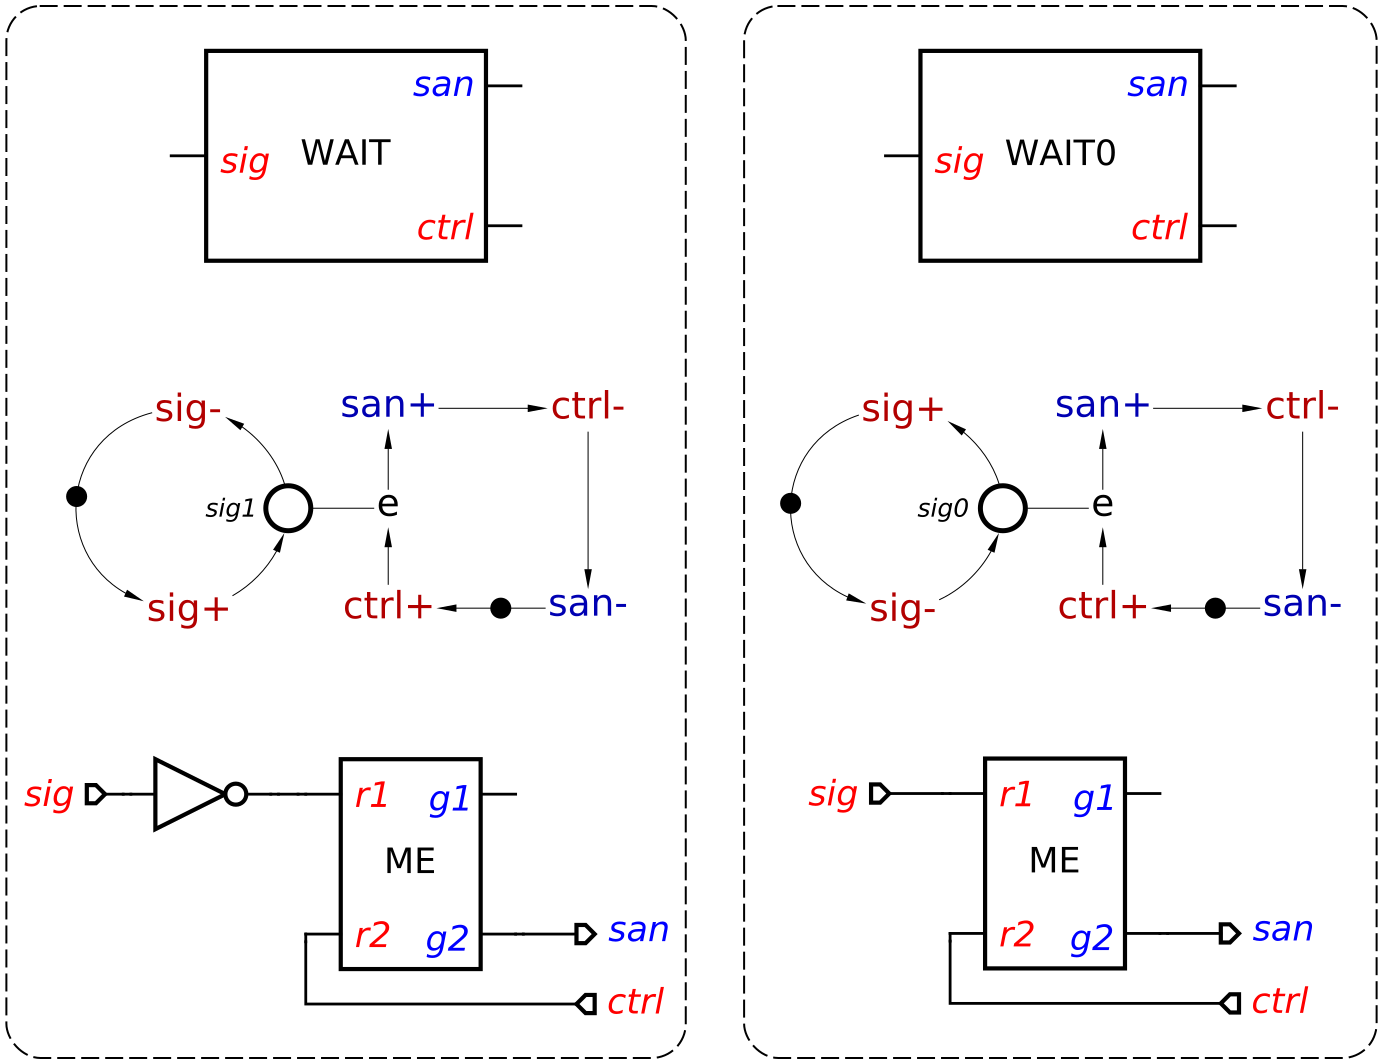
\includegraphics[scale=0.23]{fig/WAIT.pdf}
    \caption{\textsf{WAIT} and \textsf{WAIT0}: block diagram,
    specification and implementation.}
    \label{fig:wait}
\end{center}
\end{figure}

This section presents a family of \emph{decision-making} components that perform
non-trivial event arbitration and coordination tasks and rely on the previously
introduced synchronisation primitives.

\subsection{WAITX}
\subsection{WAITX2}
\subsection{SAMPLE}
\subsection{OM}

% \begin{figure}[h!]
% \begin{center}
%   \includegraphics[width=0.84\linewidth]{FIG/ope-chip.pdf}
%   \vspace{-3mm}
%   \caption{Resiliency of asynchronous control under unstable voltage.}
%   \label{fig:voltage-resiliency}
% \end{center}
% \vspace{-7mm}
% \end{figure}

\section{Conclusions}

\section*{Acknowledgements}

\bibliographystyle{unsrt}
\bibliography{publications}

\end{document}
